\section{\LaTeX - Hilfestellung} % \section stats a new numbered section
lorem ipsum dolor sit amet

% figures are used for displaying images with a caption
\begin{figure}[H]
  \centering % The image is centered
  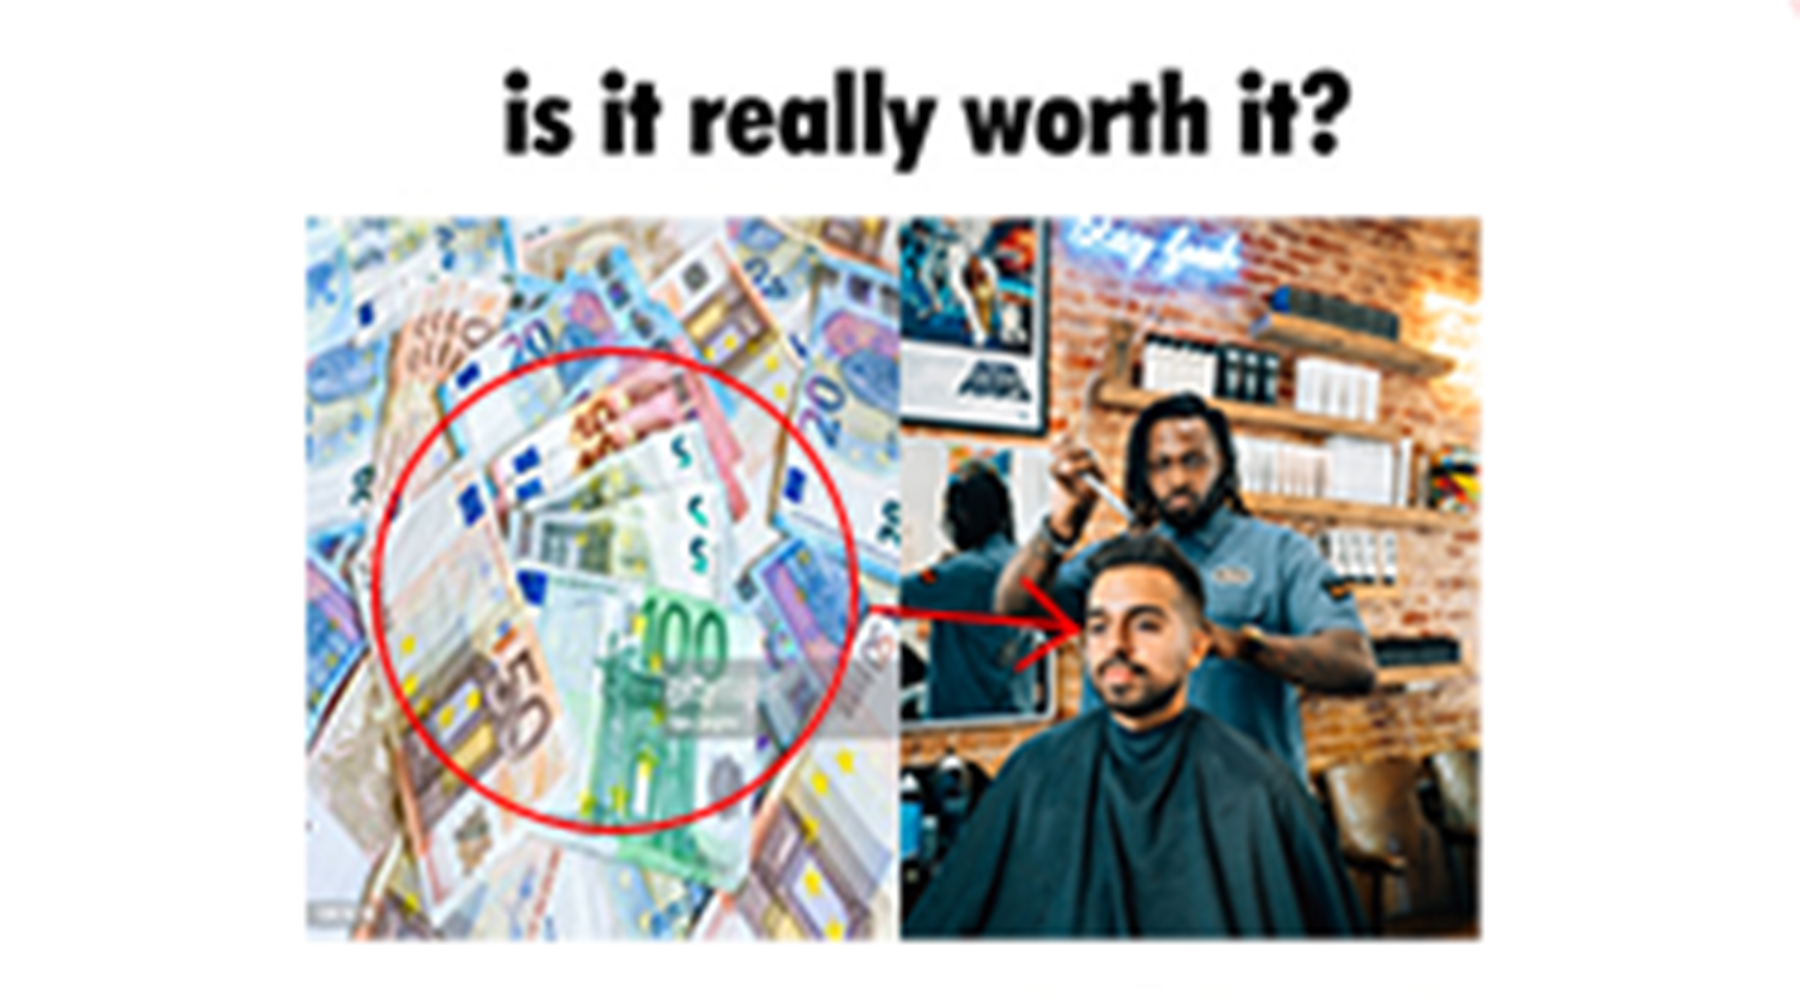
\includegraphics[width=0.75\textwidth]{images/test} % The image is imported from the file "images/test.png"
  \caption{Fahrradboxen werden von einem \ac{RBG} bedient.} % The caption of the image (\ac is used to link to an acronym)
  \label{fig:fahrrad_box} % The label of the image (used for referencing)
\end{figure}

As you can see in figure \ref{fig:fahrrad_box}, the function grows near the origin. This example is on page \pageref{fig:fahrrad_box}.

\begin{table}[H]
  \begin{center}
    \begin{tabular} { |c|c|c| }
      \hline
      cell 1 & cell 2 & cell 3 \\
      \hline
      cell 4 & cell 5 & cell 6 \\
      cell 7 & cell 8 & cell 9 \\
      \hline
    \end{tabular}
    \caption{Wichtige Tabelle \cite{cc} und \cite{stackoverflow}}.
    \label{tab:wichtige_tabelle}
  \end{center}
\end{table}

% The following lines are used to create a list
\begin{itemize}
  \item crazy item
  \item amogus
  \item more bullets
\end{itemize}

% The following lines are used to create a numbered list
\begin{enumerate}
  \item crazy item
  \item amogus
  \item more bullets
\end{enumerate}

this is a crazy math equation: $x^2 + y^2 = z^2$, it can be inline.

\begin{math}
  x^2 + y^2 = z^2
\end{math}